\documentclass[aspectratio=169]{beamer}

\usetheme{metropolis}           % Use metropolis theme
\usepackage[utf8]{inputenc}
\usepackage{graphicx}
\usepackage{eso-pic}
\usepackage{graphics}
\usepackage{tikz}
\usepackage[export]{adjustbox}
\usepackage{multicol}
\usepackage{listings}
\usepackage{helvet}
\usepackage{booktabs}
\usepackage{threeparttable}
\usepackage{marvosym}
\usepackage{hyperref}
\usepackage{soul}	% For strike-through
\usepackage{tcolorbox} % For color box

\title{Introduction to Python\\for Stata Users}
\date{}
\author{Luis Eduardo San Martin} % Name of author(s) of session here
\institute{Development Impact Evaluation (DIME) \newline The World Bank }
\setbeamercolor{background canvas}{bg=white}	% Sets background color

% The below command places the World Bank logo and DIME logo to the right corner
\titlegraphic{%
	\begin{picture}(0,0)
	\put(330,-180){\makebox(0,0)[rt]{
\includegraphics[width=3cm]{img/WB_logo}}}
	\end{picture}%
	\begin{picture}(0,0)
	\put(390,-180){\makebox(0,0)[rt]{
\includegraphics[width=1.5cm]{img/i2i}}}
	\end{picture}%
}

%%% Section page with picture of Light bulb
\makeatletter
\defbeamertemplate*{section page}{mytheme}[1][]{
	\centering
	\begin{minipage}{22em}
		\raggedright
		\usebeamercolor[fg]{section title}
		\usebeamerfont{section title}
		\par
		\ifx\insertsubsectionhead\@empty\else%
		\usebeamercolor[fg]{subsection title}%
		\usebeamerfont{subsection title}%
		\fi
		\ifstrempty{#1}{}{%
			\includegraphics[width=100mm, height=60mm]{#1}%
		}
		\\
		\insertsectionhead\\[-1ex]
		\insertsubsectionhead
		\usebeamertemplate*{progress bar in section page}
		
	\end{minipage}
	\par
	\vspace{\baselineskip}
}
\makeatother

%%% Define a command to include picture in section, 
%%% make section, and revert to old template
\newcommand{\sectionpic}[2]{
	\setbeamertemplate{section page}[mytheme][#2]
	\section{#1}
	\setbeamertemplate{section page}[mytheme]
}

%%% The command below allows for the text that contains Stata code
\lstset{ %
	backgroundcolor=\color{white},
	basicstyle=\tiny,
	breakatwhitespace=false,
	breaklines=true,
	captionpos=b,
	commentstyle=\color{green},
	escapeinside={\%*}{*)},
	extendedchars=true,
	frame=single,
	numbers=left,
	numbersep=5pt,
	numberstyle=\tiny\color{gray},
	rulecolor=\color{black},
	showspaces=false,
	showstringspaces=false,
	showtabs=false,
	stringstyle=\color{mauve},
	tabsize=2,
	title=\lstname,
	morekeywords={not,\},\{,preconditions,effects },
	deletekeywords={time}
}

%% The below command creates the ligh bulb logos in the top right corner of the 
\begin{document}
	
	
	%%%%%%%%%%%%%%%%%%%%%%%%%%%%%%%%%%%%%%%%%%% Title slide
	{
		\usebackgroundtemplate{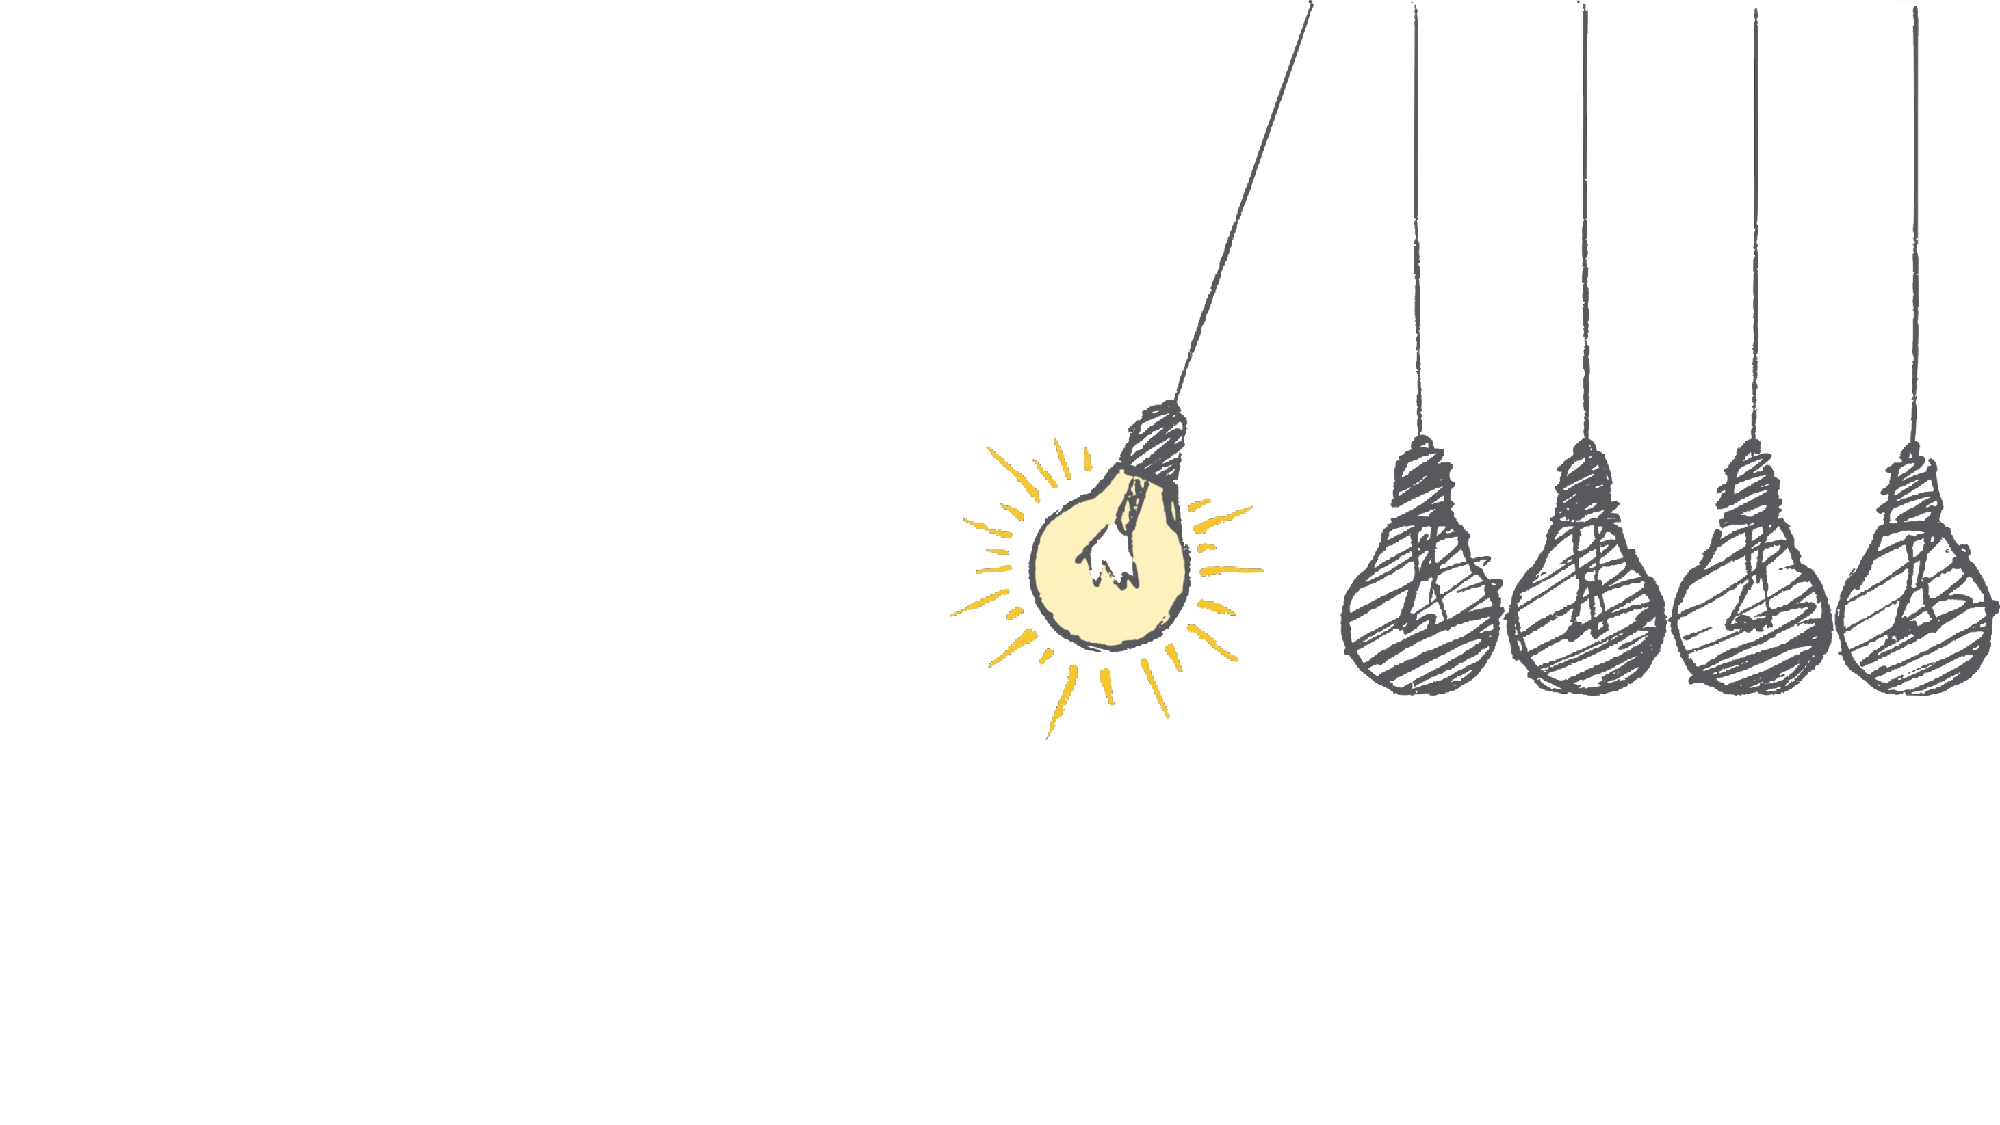
\includegraphics[height=55mm,right]{img/top_right_corner.pdf}} 
		\maketitle
	}

\begin{frame}

	\frametitle{Overview} % Table of contents slide, comment this block out to remove it
	\tableofcontents % Throughout your presentation, if you choose to use \section{} and \subsection{} commands, these will automatically be printed on this slide as an overview of your presentation

\end{frame}

%%%%%%%%%%%%%%%%%%%%%%%%%%%%%%%%%%%%%%%%%%% Section title slide
\sectionpic{Introduction}{img/section_slide}

%%%%%%%%%%%%%%%%%%%%%%%%%%%%%%%%%%%%%%%%%%% Regular slides
\begin{frame}{Introduction}

	\begin{itemize}
		\item This session will introduce you to the basics of Python
		\item In the end we will apply this to a web scraping exercise 
		\item After this session, you'll be able to write and review \textbf{basic} Python code
		\item This session does not include how to use datasets in Python 
		-- instead it will focus on the fundamental building blocks to everything in Python,
		data types
	\end{itemize}

\end{frame}

\begin{frame}{Introduction - Python for Stata users}
	
	\begin{itemize}
		\item There are many great Python courses available for free on the internet -- so why is DIME Analytics making yet another one?
		\item This session makes two assumptions not common among the courses already available:
		\begin{itemize}
			\item We assume that you will use Python for research and not computer science
			\item We assume that you are coming from a Stata background 
		\end{itemize}
		\item Many concepts will be explained by referencing concepts in Stata
	\end{itemize}
	
\end{frame}

\begin{frame}{Introduction - Why Python if I already use Stata?}

	\begin{itemize}
		\item Versatility: you can solve almost any programming task with Python:
		\begin{itemize}
			\item Web scraping, text analysis, web applications to retrieve data, machine learning
		\end{itemize}
		\item Much bigger user base
		\item Python is open source and free to use!
		\item Since it's open source it is easier to run everywhere -- for example on big data servers
	\end{itemize}

	However, a big part of the user base does not do research or data science, 
	and libraries for some less frequently used statistical operation 
	have not yet been developed

\end{frame}

%%%%%%%%%%%%%%%%%%%%%%%%%%%%%%%%%%%%%%%%%%% Section title slide
\sectionpic{Getting started}{img/section_slide}

%%%%%%%%%%%%%%%%%%%%%%%%%%%%%%%%%%%%%%%%%%% Regular slides
\begin{frame}{Getting started}

	\begin{itemize}
		\item We'll use Google Colab for this session: https://colab.research.google.com
		\item Colab is similar to a Google doc for coding, and it runs Python by default
	\end{itemize}

\end{frame}

\begin{frame}{Getting started - Colab}

	\begin{itemize}
		\item Go to https://colab.research.google.com
		\item Click on \texttt{NEW NOTEBOOK} if you're already logged in, or go to \texttt{File > New notebook} if you're not
	\end{itemize}

	\begin{multicols}{2}

		\begin{figure}
			\centering
			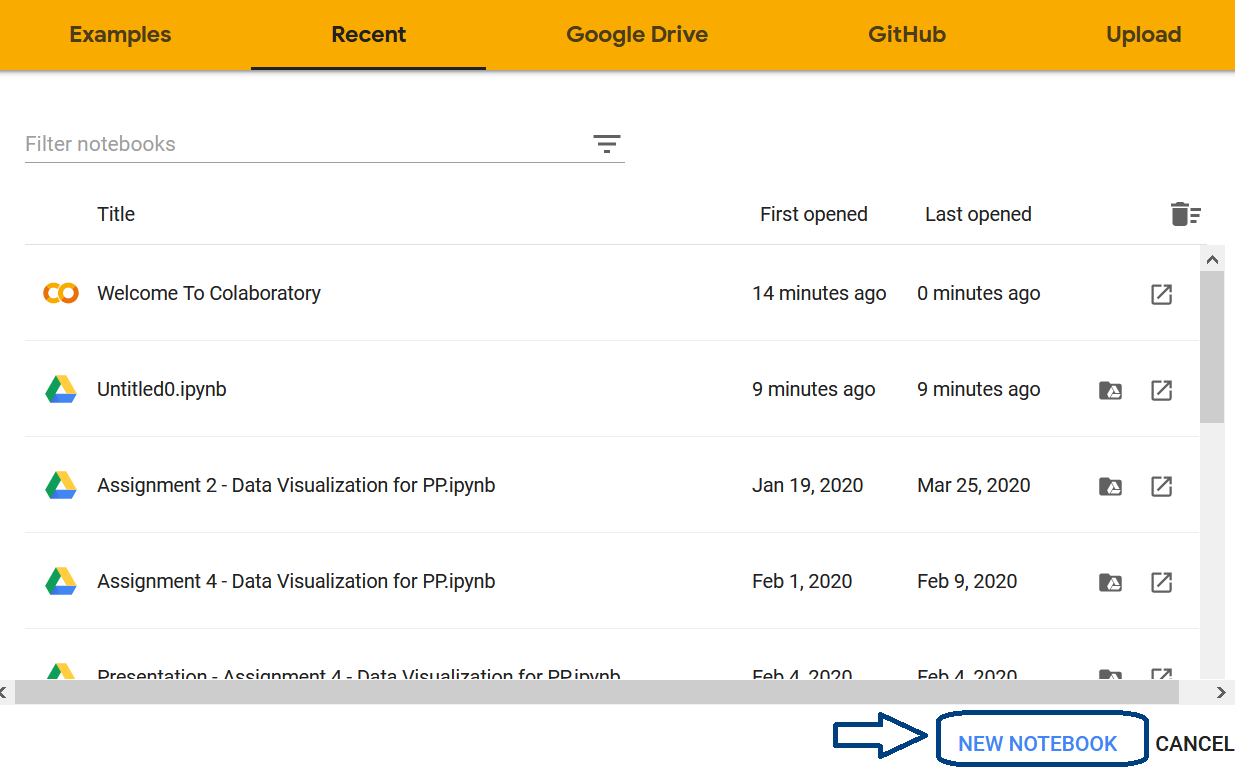
\includegraphics[width=0.9\linewidth]{img/new_nb_logged_in.png}
			\caption{Do this if you're already logged in}
		\end{figure}
		\begin{figure}
			\centering
			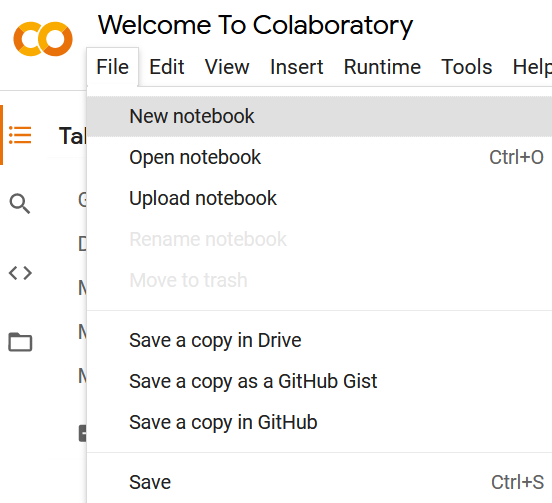
\includegraphics[width=0.6\linewidth]{img/new_nb_not_logged_in.png}
			\caption{Do this if you're not -- you'll be prompted to log in}
		\end{figure}

	\end{multicols}

\end{frame}

\begin{frame}{Getting started - Colab}

	You should end up with something like this in your browser:

	\begin{figure}
		\centering
		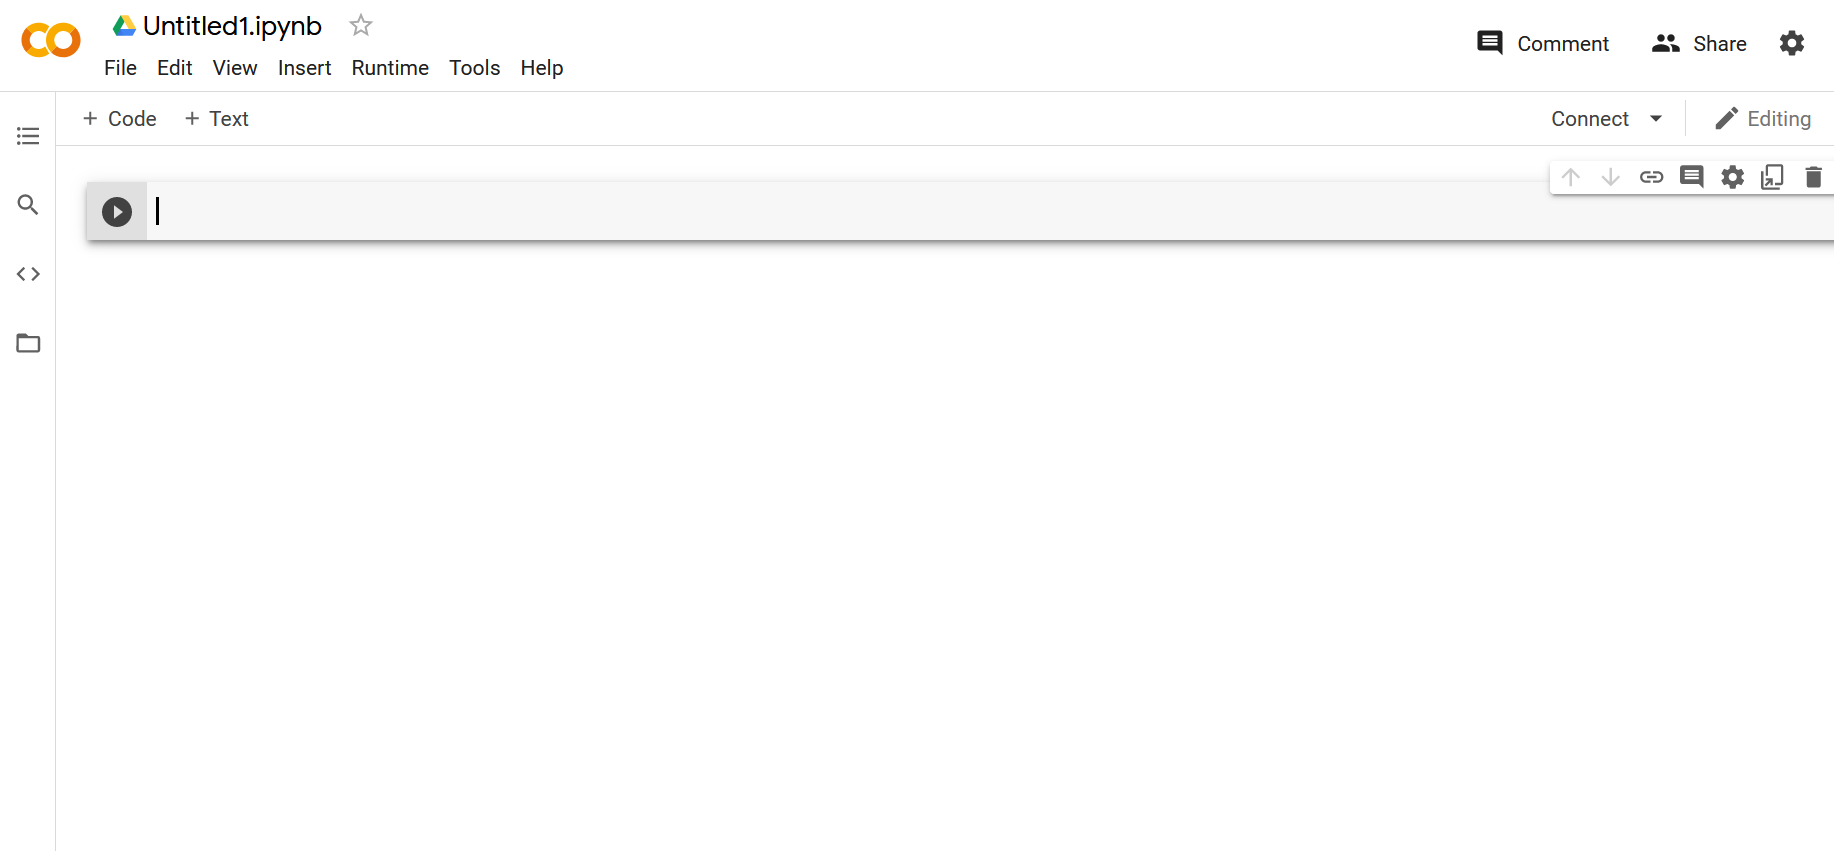
\includegraphics[width=0.9\linewidth]{img/colab.png}
	\end{figure}

\end{frame}

\begin{frame}{Getting started - Colab}

	\begin{itemize}
		\item Colab organizes code in blocks -- each block is like its own script
		\item To run the code in a block, 
		click the $\blacktriangleright$ symbol or press \texttt{Ctrl} + \texttt{Enter}
	\end{itemize}

	\begin{figure}
		\centering
		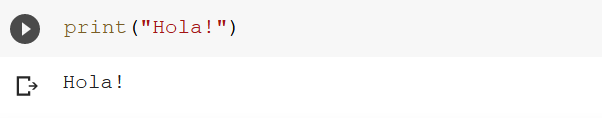
\includegraphics[width=0.6\linewidth]{img/block_of_code.png}
	\end{figure}

\end{frame}

\begin{frame}{Getting started - Colab}

	\begin{itemize}
		\item Click on \texttt{+ Code} to add new blocks of code
	\end{itemize}

	\begin{figure}
		\centering
		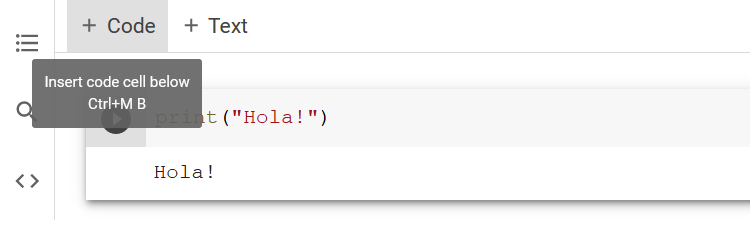
\includegraphics[width=0.6\linewidth]{img/add_code.png}
	\end{figure}	

	\textbf{Important:} Code blocks are a feature specific to Colab. Most Python distributions don't have this feature

\end{frame}

%%%%%%%%%%%%%%%%%%%%%%%%%%%%%%%%%%%%%%%%%%% Section title slide
\sectionpic{Python variables}{img/section_slide}

%%%%%%%%%%%%%%%%%%%%%%%%%%%%%%%%%%%%%%%%%%% Regular slides
\begin{frame}{Python variables}

	\begin{itemize}
		\item In Stata, variables are columns of a dataframe
		\item In Python, variables are everything that we define with a name to be referenced -- more similar to Stata's locals or globals (macros)
		\item Nonetheless, while macros in Stata are "nice to have" and useful, variables in Python are the building block of everything and you cannot write code without them
		\item Variables are also broader than locals, globals or columns in Stata; for example, functions and datasets can be a variable in Python
	\end{itemize}

\end{frame}

\begin{frame}{Python variables}

	Just like in Stata, in Python we use the \texttt{=} operator to create variables

	\begin{figure}
		\centering
		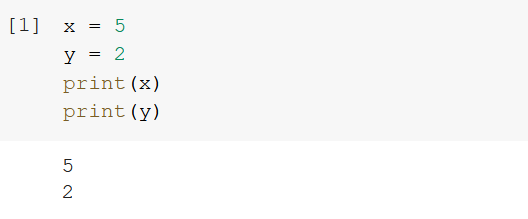
\includegraphics[width=0.6\linewidth]{img/assignation.png}
	\end{figure}

\end{frame}

\begin{frame}{Python variables}

	This also works when we're trying to replace an existing variable

	\begin{figure}
		\centering
		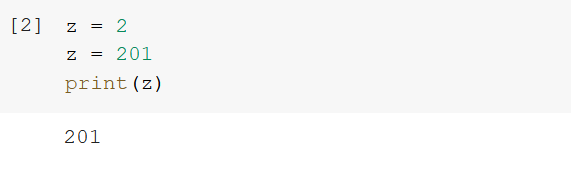
\includegraphics[width=0.6\linewidth]{img/replace.png}
	\end{figure}

\end{frame}

%%%%%%%%%%%%%%%%%%%%%%%%%%%%%%%%%%%%%%%%%%% Section title slide
\sectionpic{Python basic data types}{img/section_slide}

%%%%%%%%%%%%%%%%%%%%%%%%%%%%%%%%%%%%%%%%%%% Regular slides
\begin{frame}{Python basic data types}

	\begin{itemize}
		\item Every Python variable has a data type
	\end{itemize}

	\begin{figure}
		\centering
		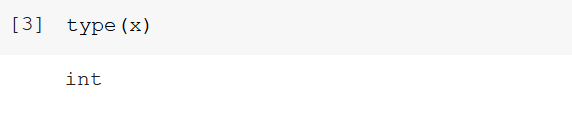
\includegraphics[width=0.6\linewidth]{img/data_type.png}
	\end{figure}

	\begin{itemize}
		\item Today we will cover the most basic data types: 
		int/float (numbers), strings, booleans and lists
		\item Variables in Python do more than just store data.
		They provide operations related to their data type, 
		for example: add and remove item from a list, make a string upper case, etc.
	\end{itemize}

\end{frame}

\begin{frame}{Python - more on data types}

	\begin{itemize}
		\item Python has thousands of other data types
		\item This is because users can build their own data types based on the built-in types 
		-- you will frequently use such data types \scriptsize(and we'll use some of them later today) \normalsize
		\item For example, a dataset in Python is a variable from the \texttt{pandas dataset} type, a custom data type implemented by the Python community
		\item All of these custom data types store data 
		and provide built-in functionality specially implemented for the intended context
	\end{itemize}
\end{frame}

\begin{frame}{Python basic data types - \texttt{int}}

	The \texttt{x} and \texttt{y} variables we just defined have the data type \texttt{int}

	\begin{figure}
		\centering
		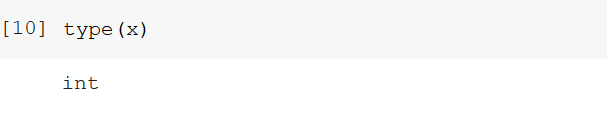
\includegraphics[width=0.6\linewidth]{img/type_int.png}
	\end{figure}

	\texttt{int} variables are integer numbers. We can do mathematical operations with them
	\begin{figure}
		\centering
		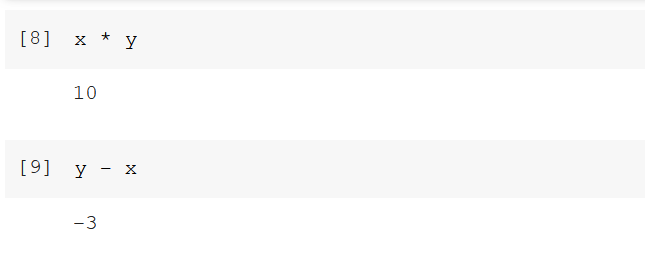
\includegraphics[width=0.6\linewidth]{img/math_integers.png}
	\end{figure}

\end{frame}

\begin{frame}{Python basic data types - \texttt{float}}

	\texttt{float} variables, on the other hand, represent real numbers 
	-- we can do mathematical operations with floats as well

	\begin{figure}
		\centering
		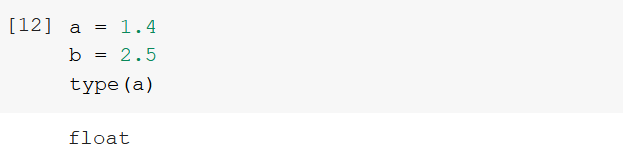
\includegraphics[width=0.6\linewidth]{img/type_float.png}
	\end{figure}

	\begin{itemize}	
		\item Python is what's called "\textit{dynamically typed}", 
	which means that you do not need to indicate what data type you want
		\item It detects when a variable is an integer, floating point (decimal number), 
	text, etc. as long as it is a built-in data type.
	\end{itemize}

\end{frame}

\begin{frame}{Python basic data types - \texttt{str}}

	\texttt{str} variables are strings with text

	\begin{figure}
		\centering
		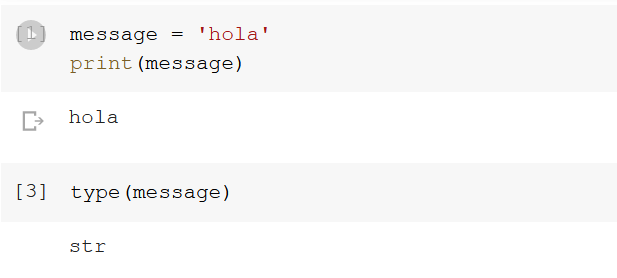
\includegraphics[width=0.6\linewidth]{img/string_type.png}
	\end{figure}

	\textbf{Note:} A variable can be used across code blocks 
	-- this is common in all notebook styled python interfaces, like Colab

\end{frame}

\begin{frame}{Python basic data types - \texttt{str}}

	Python allows two types of "mathematical" operations with \texttt{str}: \texttt{+} and \texttt{*}

	\begin{figure}
		\centering
		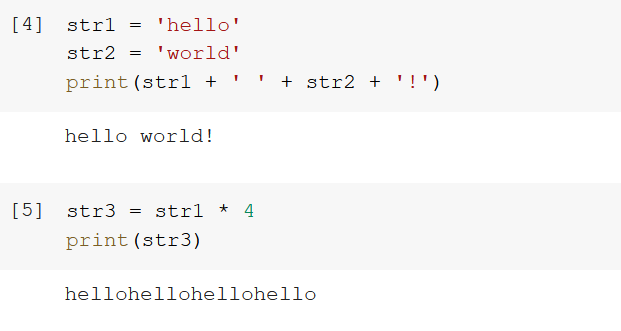
\includegraphics[width=0.6\linewidth]{img/string_operations.png}
	\end{figure}

\end{frame}

\begin{frame}{Python basic data types - Lists}

	\begin{itemize}
		\item A list is a variable that groups other variables
		\item Lists can have different data types in them at the same time. They can even include other lists!
		\item Lists are defined enclosed in brackets and separating its values with commas
	\end{itemize}

	\begin{figure}
		\centering
		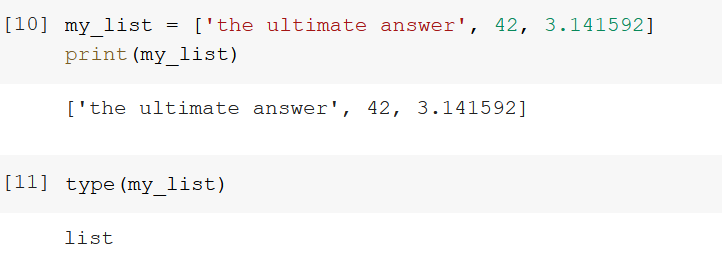
\includegraphics[width=0.8\linewidth]{img/list_type.png}
	\end{figure}

\end{frame}

\begin{frame}{Python basic data types - Lists}

	We can index lists

	\begin{figure}
		\centering
		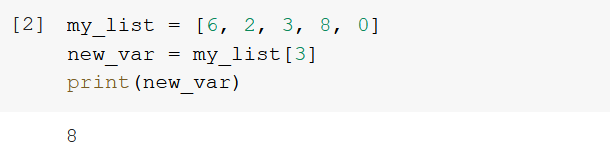
\includegraphics[width=0.6\linewidth]{img/list_index.png}
	\end{figure}

	\textbf{Important:} Python starts indexing at zero, not at one

\end{frame}

\begin{frame}{Python basic data types - Lists}

	We can subset lists

	\begin{figure}
		\centering
		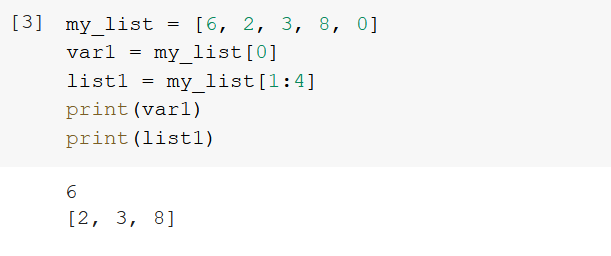
\includegraphics[width=0.6\linewidth]{img/list_subset.png}
	\end{figure}

	\textbf{Important:} When subsetting a list with \texttt{[a:b]}, Python will include the element at position \texttt{a} \textbf{but will exlude the one at position \texttt{b}}
	\newline \scriptsize hence \texttt{my\_list[1:4]} returns the elements at positions 1, 2, 3 \normalsize

\end{frame}

\begin{frame}{Python basic data types - Lists}

	We can also use negative indices: they represent the elements of a list starting by the end

	\begin{figure}
		\centering
		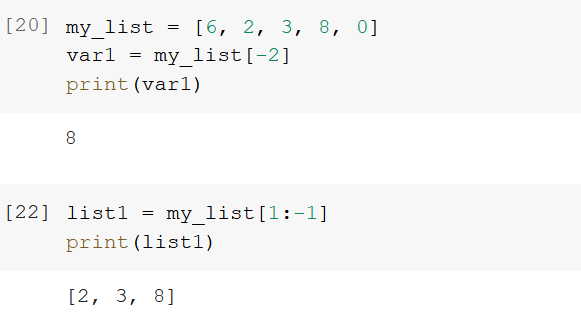
\includegraphics[width=0.6\linewidth]{img/list_subset_negative.png}
	\end{figure}

\end{frame}

\begin{frame}{Python basic data types - Lists}

	To add new elements to existing lists, we use \texttt{.append()}

	\begin{figure}
		\centering
		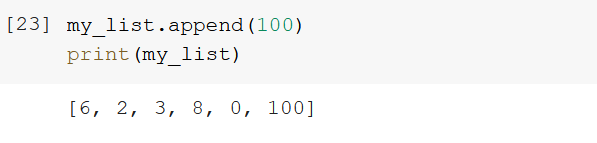
\includegraphics[width=0.6\linewidth]{img/list_append.png}
	\end{figure}

	Note that this will modify our list variable in-place -- it's not necessary to define the result as a new variable with \texttt{=} when we use \texttt{.append()}

\end{frame}

\begin{frame}{Python basic data types - Lists}

	We can use the \texttt{+} and \texttt{*} operators with lists

	\begin{figure}
		\centering
		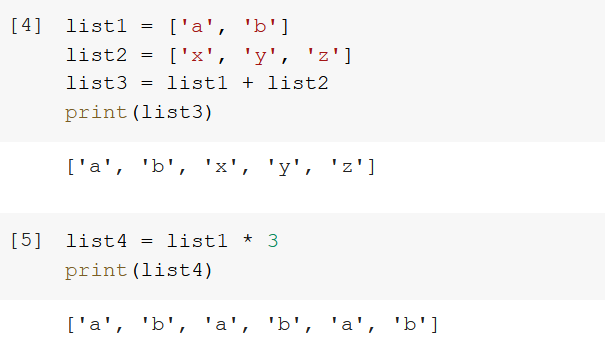
\includegraphics[width=0.6\linewidth]{img/list_operations.png}
	\end{figure}

\end{frame}

\begin{frame}{Python basic data types - Booleans}

	Booleans (\texttt{bool}) are variables representing boolean values -- either \texttt{True} or \texttt{False}

	\begin{figure}
		\centering
		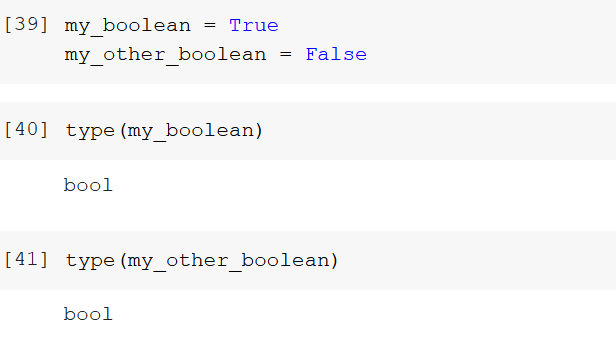
\includegraphics[width=0.6\linewidth]{img/bool.png}
	\end{figure}

\end{frame}

\begin{frame}{Python basic data types - Booleans}

	\begin{itemize}	
		\item We can create booleans by direct assignation or with boolean expressions
		\item When using direct assignation, Python recognizes booleans when they are written without quotes and with the first character in uppercase and the rest in lowercase
	\end{itemize}

	\begin{figure}
		\centering
		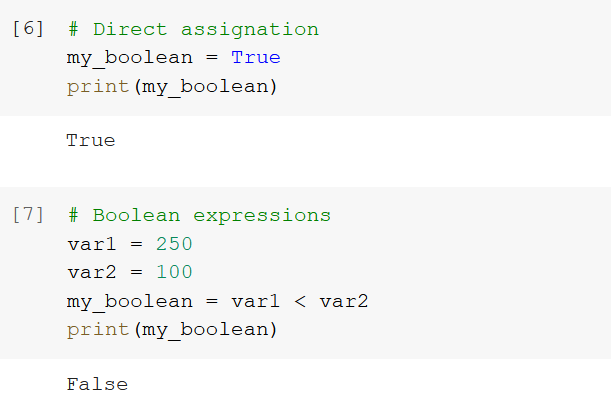
\includegraphics[width=0.5\linewidth]{img/bool_assignation.png}
	\end{figure}

\end{frame}

\begin{frame}{Python basic data types - Booleans}

	Some operators for boolean expressions are \texttt{==}, \texttt{>}, \texttt{>=}, \texttt{<}, \texttt{<=}, and \texttt{in} (to check if an element is part of a list)

	\begin{figure}
		\centering
		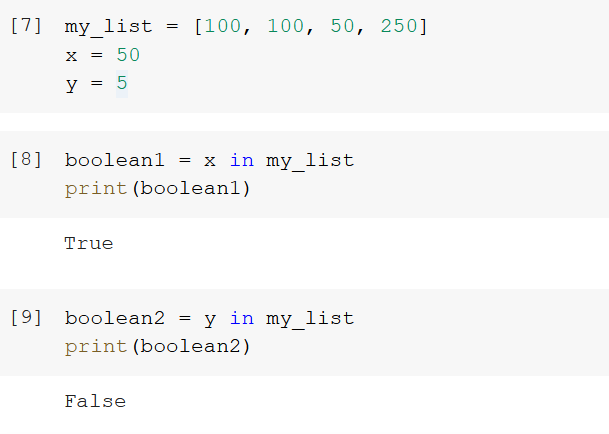
\includegraphics[width=0.6\linewidth]{img/bool_in.png}
	\end{figure}

\end{frame}

\begin{frame}{Python basic data types - Booleans}

	We can do logical operations with booleans using \texttt{and}, \texttt{or}

	\begin{multicols}{2}

		\begin{figure}
			\centering
			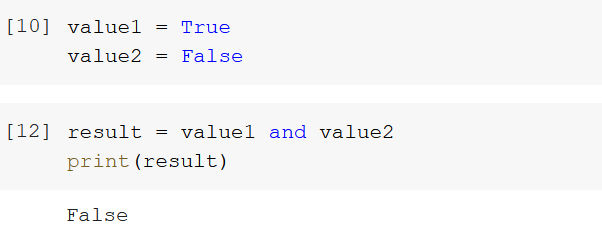
\includegraphics[width=\linewidth]{img/and.png}
		\end{figure}
		\begin{figure}
			\centering
			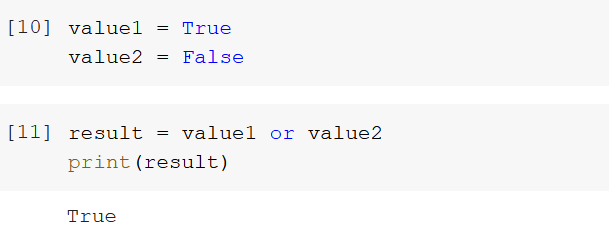
\includegraphics[width=\linewidth]{img/or.png}
		\end{figure}

	\end{multicols}

\end{frame}

\begin{frame}{Python basic data types}

	\begin{itemize}
		\item Until now, we've reviewed what Python variables and basic data types are
		\item Importantly, these are the building blocks of everything you do in Python
		\item It is simply impossible to do perform any task if you do not know how to work with the basic data types first
	\end{itemize}

\end{frame}

%%%%%%%%%%%%%%%%%%%%%%%%%%%%%%%%%%%%%%%%%%% Section title slide
\sectionpic{Python basic syntax}{img/section_slide}

%%%%%%%%%%%%%%%%%%%%%%%%%%%%%%%%%%%%%%%%%%% Regular slides

\begin{frame}{Basic syntax - Attributes}

	\begin{itemize}
		\item Attributes are very often used when programming in Python
		\item They do one of two things:
			\begin{enumerate}
				\item Attributes transform a variable in-place
				\begin{itemize}
					\item For example: \texttt{.append()}, an attribute of list variables
				\end{itemize}
			\end{enumerate}
	\end{itemize}

	\begin{figure}
		\centering
		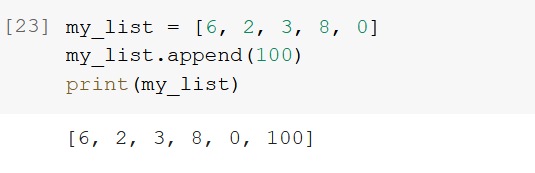
\includegraphics[width=0.6\linewidth]{img/attributes_append.png}
	\end{figure}

\end{frame}

\begin{frame}{Basic syntax - Attributes}

	2. Other attributes, by contrast, return a transformation of a variable without modifying the original
		
	\begin{itemize}
		\item For example: \texttt{.lower()} and \texttt{upper()}, attributes of string variables
	\end{itemize}

	\begin{figure}
		\centering
		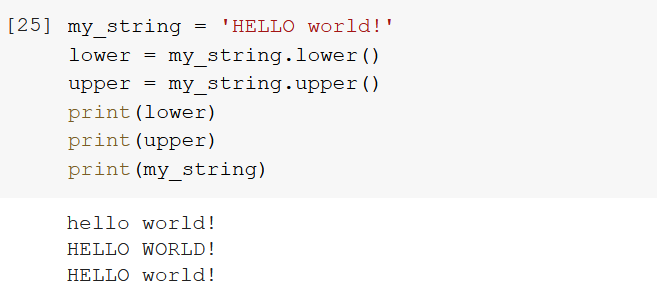
\includegraphics[width=0.6\linewidth]{img/string_lower_upper.png}
	\end{figure}

\end{frame}

\begin{frame}{Basic syntax - Attributes}

	\begin{itemize}
		\item Each data type has specific attributes. They relate to the built-in functionalities each data type has
		\item The syntax of attributes is \textit{almost} always: \texttt{VARIABLE\_NAME.ATTRIBUTE\_NAME(INPUTS\_IF\_ANY)}
	\end{itemize}

\end{frame}

\begin{frame}{Basic syntax - Looping}

	\begin{itemize}
		\item Many data types in Python belong to a group called iterables -- variables you can loop through
		\item Lists are the most commonly used iterable: if we put a list in a loop, Python will loop through every one of its elements
		\item \texttt{int} and \texttt{float} are examples of non-iterable data types
	\end{itemize}

\end{frame}

\begin{frame}{Basic syntax - Looping}

	\begin{figure}
		\centering
		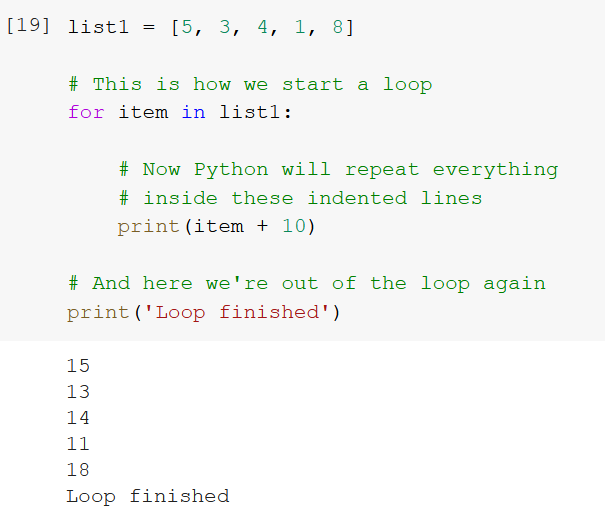
\includegraphics[width=0.6\linewidth]{img/list_loop.png}
	\end{figure}

\end{frame}

\begin{frame}{Basic syntax - Looping}

	\textbf{Important:}

	Python knows what is inside the loop and where it ends with an indentation space -- it works similar to the \texttt{\{ \}} symbols you use to open and close a loop in Stata

	\begin{multicols}{2}

		\begin{figure}
			\centering
			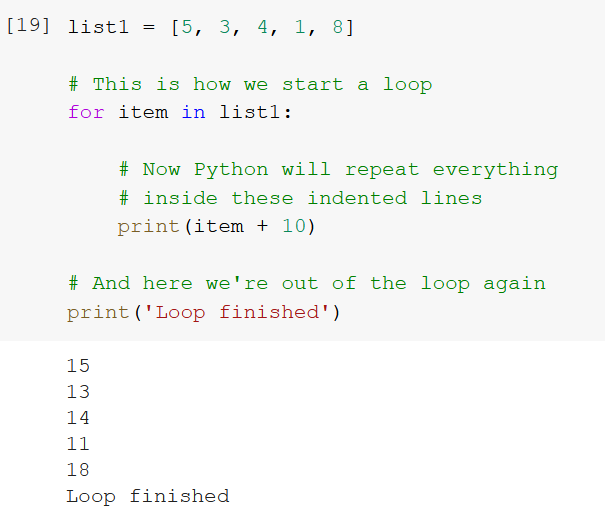
\includegraphics[width=0.86\linewidth]{img/list_loop.png}
		\end{figure}

		\begin{figure}
			\centering
			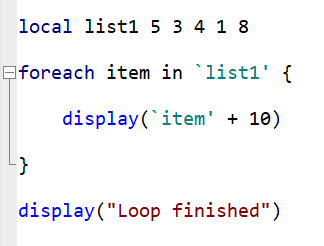
\includegraphics[width=0.55\linewidth]{img/loop_stata.png}
		\end{figure}

	\end{multicols}

\end{frame}

\begin{frame}{Basic syntax - Looping}

	\textbf{Important:}

	\begin{multicols}{2}
	
		\begin{itemize}
			\item Indentation can have two or four spaces depending on your Python interface. In any case, you can also press the \texttt{tab} key to create indented space
			\item If you ever run the script of a colleague who uses different indentation, Python will automatically know the correct one. All that matters is that indentation is consistent within the same script
		\end{itemize}
		\begin{figure}
			\centering
			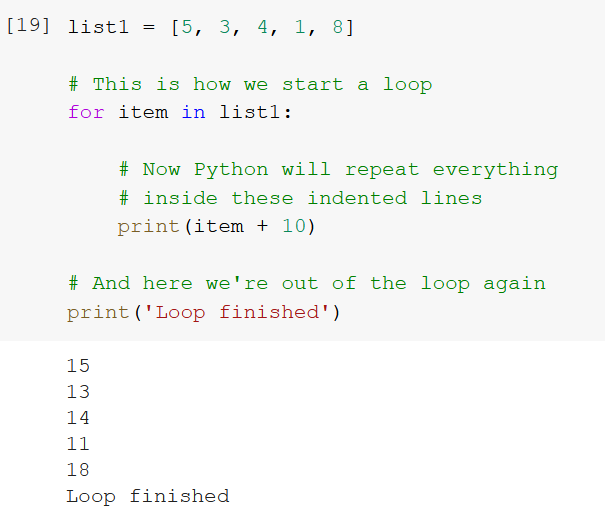
\includegraphics[width=\linewidth]{img/list_loop.png}
		\end{figure}

	\end{multicols}

\end{frame}

\begin{frame}{Basic syntax - Looping}

	Strings are also iterables: Python loops through every character with them

	\begin{figure}
		\centering
		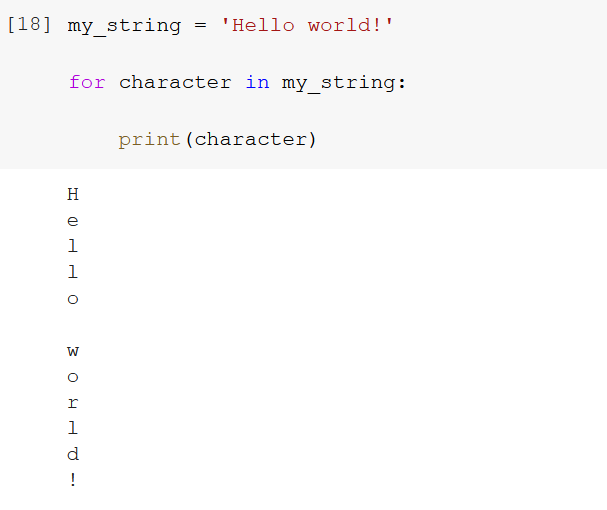
\includegraphics[width=0.55\linewidth]{img/string_loop.png}
	\end{figure}

\end{frame}

%%%%%%%%%%%%%%%%%%%%%%%%%%%%%%%%%%%%%%%%%%% Section title slide
\sectionpic{Annex}{img/section_slide}

%%%%%%%%%%%%%%%%%%%%%%%%%%%%%%%%%%%%%%%%%%% Regular slides

\begin{frame}{Python basic data types - Tuples}

	Tuples are lists of variables. They are defined in parentheses and separate their elements by commas.

	\begin{figure}
		\centering
		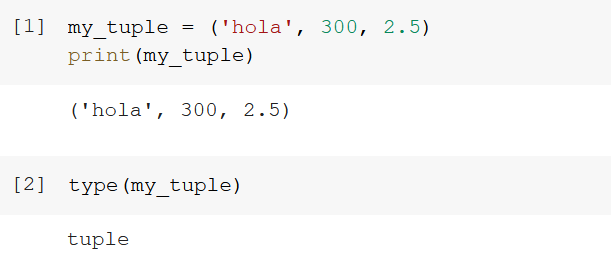
\includegraphics[width=0.55\linewidth]{img/tuple.png}
	\end{figure}

\end{frame}

\begin{frame}{Python basic data types - Tuples}

	Tuples are very similar to lists in that both use indices and subsets

	\begin{figure}
		\centering
		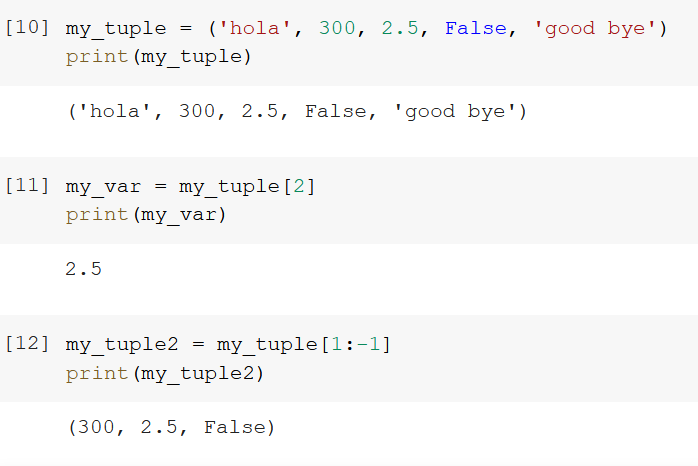
\includegraphics[width=0.55\linewidth]{img/tuple_index_subset.png}
	\end{figure}

\end{frame}

\begin{frame}{Python basic data types - Tuples}


	The crucial difference between them is that tuples are inmutable: once defined, we can't add new elements to them or replace the existing ones

	\begin{figure}
		\centering
		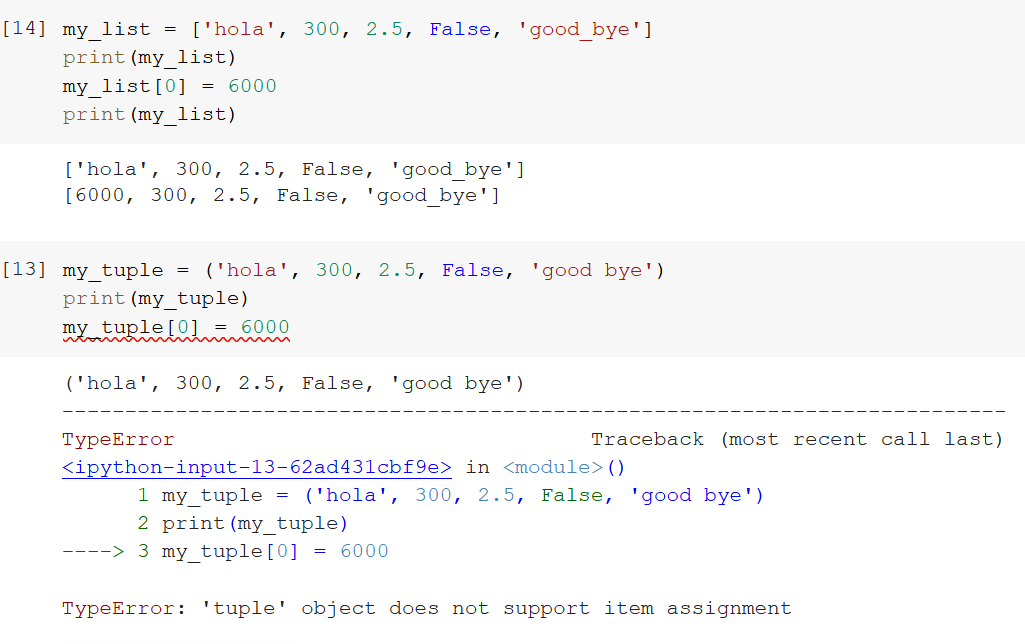
\includegraphics[width=0.55\linewidth]{img/tuple_error.png}
	\end{figure}

\end{frame}

\begin{frame}{Basic syntax - Conditional expressions}

       \textbf{Conditional expressions:}
	\texttt{if}, \texttt{elif}, and \texttt{else} are used to define conditional operations. They also use idented space

	\begin{multicols}{3}

		\begin{figure}
			\centering
			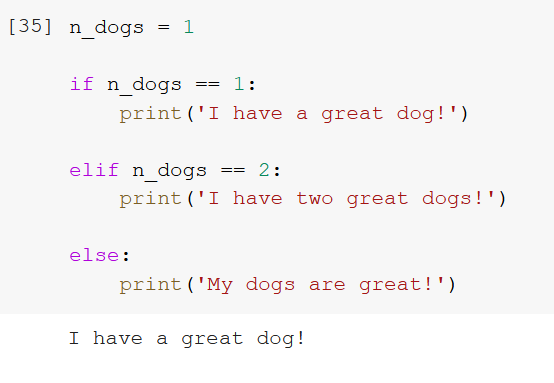
\includegraphics[width=\linewidth]{img/if.png}
		\end{figure}
		\begin{figure}
			\centering
			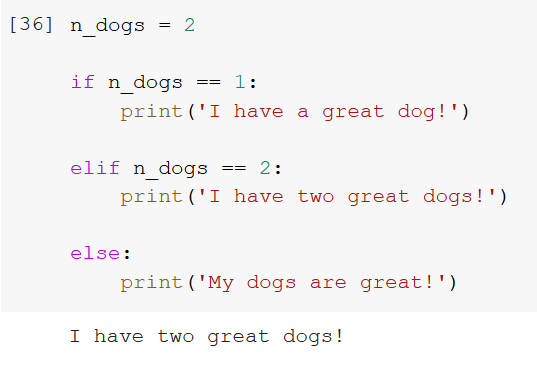
\includegraphics[width=\linewidth]{img/elif.png}
		\end{figure}
		\begin{figure}
			\centering
			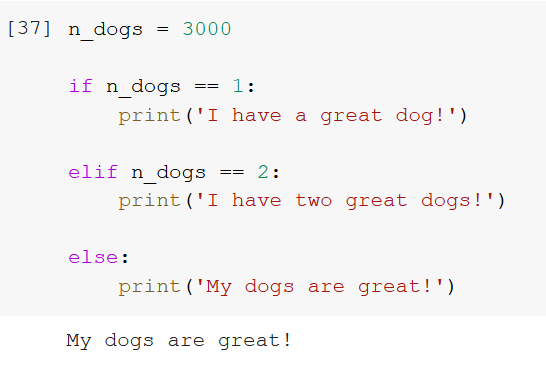
\includegraphics[width=\linewidth]{img/else.png}
		\end{figure}

	\end{multicols}

\end{frame}

\begin{frame}{Basic syntax - Conditional expressions}

	\begin{itemize}
		\item Instead of a boolean expression we can use a boolean value with \texttt{if} or \texttt{elif}
		\item \texttt{if} doesn't necessarily need to be used with \texttt{elif} of with \texttt{else}, we can use it alone
	\end{itemize}

	\begin{multicols}{2}

		\begin{figure}
			\centering
			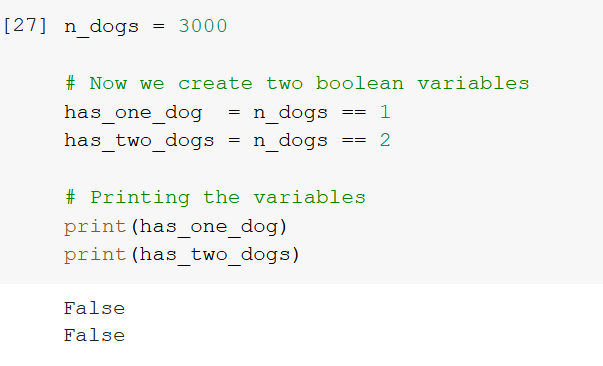
\includegraphics[width=\linewidth]{img/boolean_variables.png}
		\end{figure}
		\begin{figure}
			\centering
			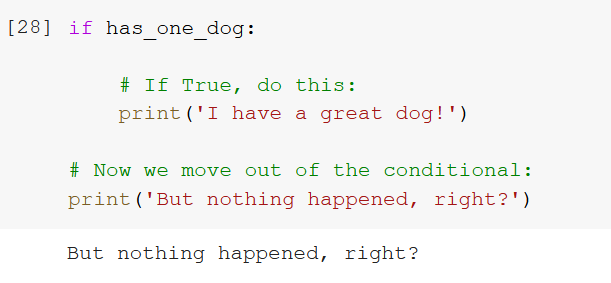
\includegraphics[width=\linewidth]{img/if_alone.png}
		\end{figure}

	\end{multicols}

\end{frame}

\begin{frame}{Basic syntax - Conditional expressions}

	We can also use \texttt{if} and \texttt{elif} without \texttt{else}

	\begin{multicols}{2}

		\begin{figure}
			\centering
			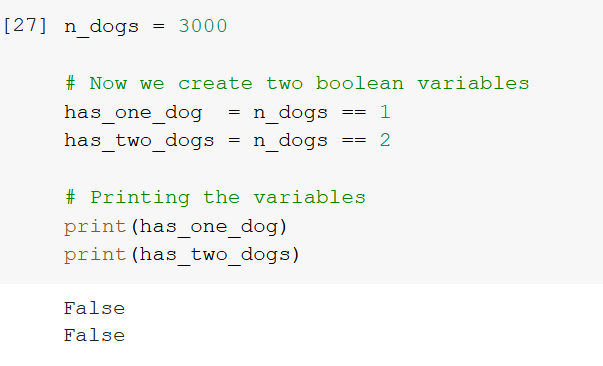
\includegraphics[width=\linewidth]{img/boolean_variables.png}
		\end{figure}
		\begin{figure}
			\centering
			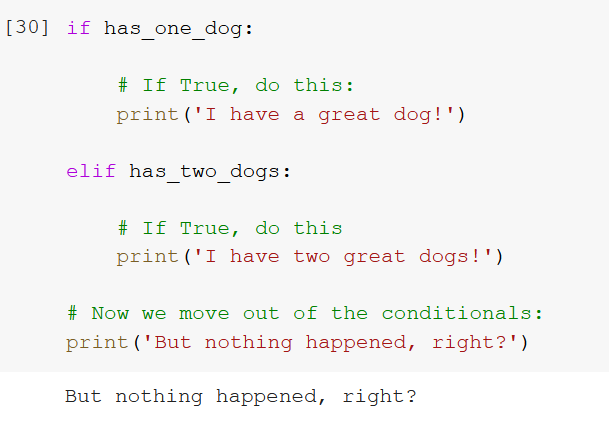
\includegraphics[width=\linewidth]{img/if_elif.png}
		\end{figure}

	\end{multicols}

\end{frame}

\begin{frame}{Basic syntax - Conditional expressions}

	And we can use \texttt{if} and \texttt{else} without \texttt{elif}

	\begin{multicols}{2}

		\begin{figure}
			\centering
			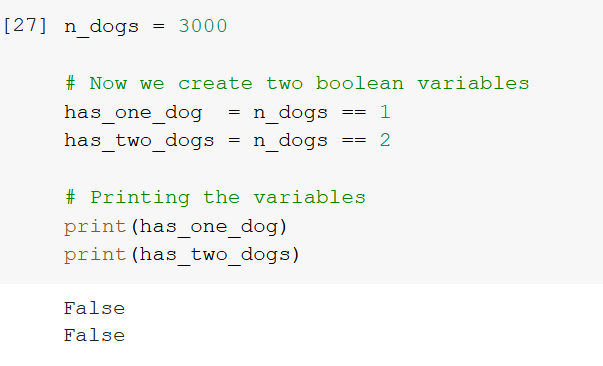
\includegraphics[width=\linewidth]{img/boolean_variables.png}
		\end{figure}
		\begin{figure}
			\centering
			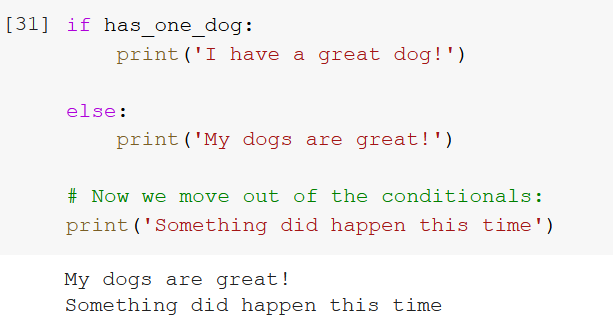
\includegraphics[width=\linewidth]{img/if_else.png}
		\end{figure}

	\end{multicols}

\end{frame}

\begin{frame}{Basic syntax - Conditional expressions}

	\begin{itemize}
		\item If a boolean expression returned \texttt{True} for conditions in both \texttt{if} and \texttt{elif}, only the operations  under \texttt{if} would be executed
		\item If more than one boolean expression under several \texttt{elif} conditions were to return \texttt{True}, only the operations under the first \texttt{elif} condition evaluated to \texttt{True} would be executed
	\end{itemize}

	\begin{multicols}{2}

		\begin{figure}
			\centering
			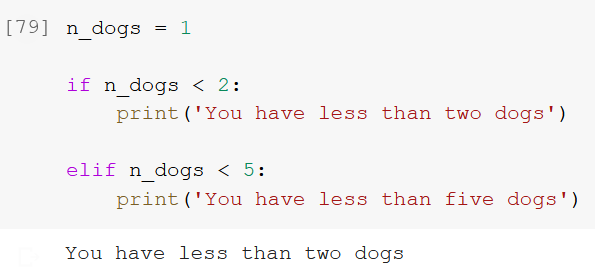
\includegraphics[width=\linewidth]{img/if_and_elif_true.png}
		\end{figure}
		\begin{figure}
			\centering
			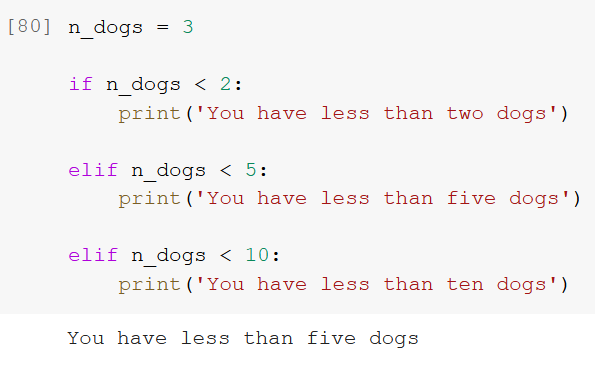
\includegraphics[width=\linewidth]{img/elif_and_elif_true.png}
		\end{figure}

	\end{multicols}

\end{frame}

\end{document}
